%!TEX root = ../thesis.tex
\chapter{\KThinning \DQL Analysis}\label{k-thinning-dql-analysis} 


\section*{Hyperparameter Analysis}


\begin{table}[ht]
\begin{center}
\begin{tabular}{lcc}
 \textbf{Hyperparameter} & \textbf{Importance} & \textbf{Correlation} \\
 \addlinespace[0.2cm]
 \texttt{optimise\_freq} & \Progress{0.138}{blue} & \Progress{0.42}{red} \\
 \texttt{target\_update\_freq} & \Progress{0.133}{blue} & \Progress{0.124}{green} \\
 \texttt{eps\_decay} & \Progress{0.088}{blue} & \Progress{0.051}{red} \\
 \texttt{pre\_train\_episodes} & \Progress{0.084}{blue} & \Progress{0.293}{green} \\
 \texttt{batch\_size} & \Progress{0.074}{blue} & \Progress{0.205}{red} \\
\end{tabular}
\caption{\KThinning hyperparameter importance~\cite{biewald2020wandb} for $n=20$, $m=400$.}
\label{k-thinning-hyperparameter-analysis}
\end{center}
\end{table}


We can observe in Table~\ref{k-thinning-hyperparameter-analysis} that the normalised load domain trick is not as crucial for \KThinning as it was for \TwoThinning\NOTE{A}{Mention some bullshit possible reason?}. On the other hand, the analysis suggests more frequent optimisation update steps and more curriculum learning (pretraining) episodes. 


\section*{Training}


\begin{figure}[ht]
    \centering
    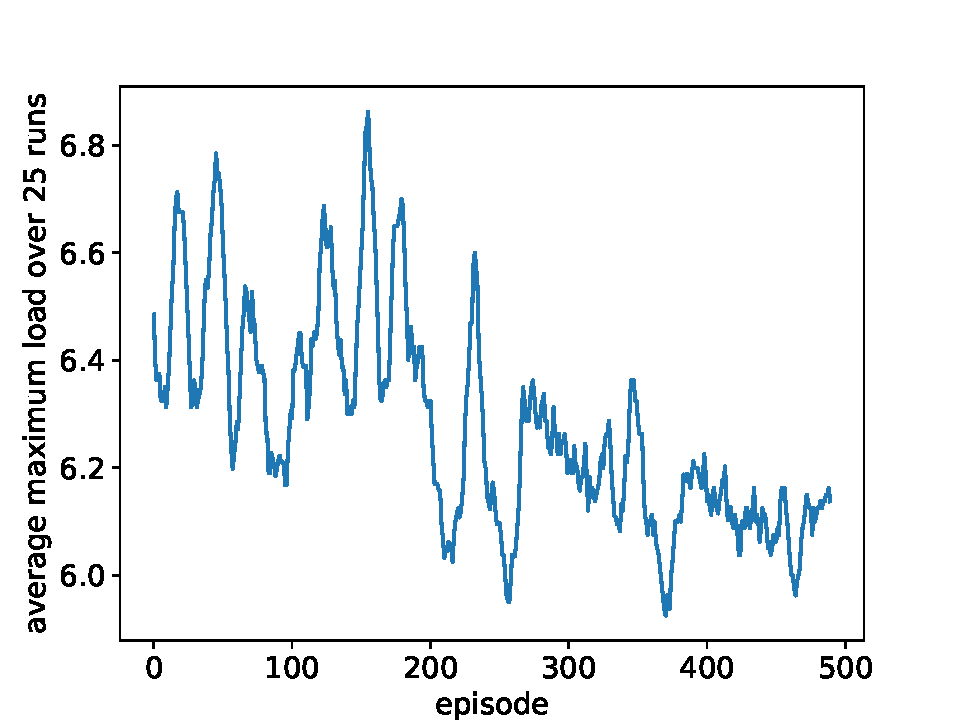
\includegraphics[scale=0.6]{Chapter4/Figs/training_progression_rolling_window_5_25_3.pdf}
    \caption{\KThinning training curve for $n=5$, $m=25$, $k=3$, with $10$ episodes wide rolling window averaging for readability purposes.}
    \label{k-thinning-training-curve}
\end{figure}


The training progression shown in Figure~\ref{k-thinning-training-curve} is similar to that of \TwoThinning. We can also observe that after reaching a new best score, the agent requires many more episodes to consistently settle below this score.
